\chapter{Réalisation}

\section*{Introduction}
La phase de réalisation concrétise l'ensemble des études préalables et conceptuelles effectuées. Ce chapitre présente les aspects techniques de la mise en œuvre du système "Central de Réclamation", depuis la configuration de l'environnement de développement jusqu'à la présentation des interfaces utilisateurs finales, en passant par l'architecture logicielle retenue.

\section{Environnement de réalisation}
Pour concrétiser ce projet, nous avons mis en place un environnement de développement complet.

\subsection{Outils logiciels}
\begin{itemize}
    \item \textbf{Visual Studio Code :} Notre environnement de développement intégré (IDE) principal.
    \item \textbf{XAMPP :} Pour simuler un serveur de production en local (Apache/MySQL/PHP).
    \item \textbf{Git :} Pour le versionnage du code source.
    \item \textbf{PHPMailer :} Bibliothèque d'envoi d'emails SMTP.
\end{itemize}

\section{Architecture de l'application}
L'application repose sur une architecture MVC (Modèle-Vue-Contrôleur) simplifiée :
\begin{itemize}
    \item \textbf{Modèle :} Gestion des données (fichiers dans \texttt{/api/} et \texttt{/config/}).
    \item \textbf{Vue :} Interfaces utilisateurs (fichiers dans \texttt{/pages/}).
    \item \textbf{Contrôleur :} Logique métier et routage (fichier \texttt{index.php}).
\end{itemize}

\section{Interfaces Graphiques}
L'ergonomie a été travaillée pour offrir une expérience utilisateur fluide et professionnelle. Nous présentons ci-dessous les principales interfaces du système, organisées par espace utilisateur.

% ==================================================
% ESPACE CLIENT
% ==================================================
\subsection{Espace Client}

\subsubsection{Page d'Accueil et Authentification}
La page d'accueil permet aux utilisateurs (Clients et Personnel) de se connecter de manière sécurisée. Le design est épuré, aux couleurs de l'entreprise (Bleu et Blanc).

\begin{figure}[H]
    \centering
    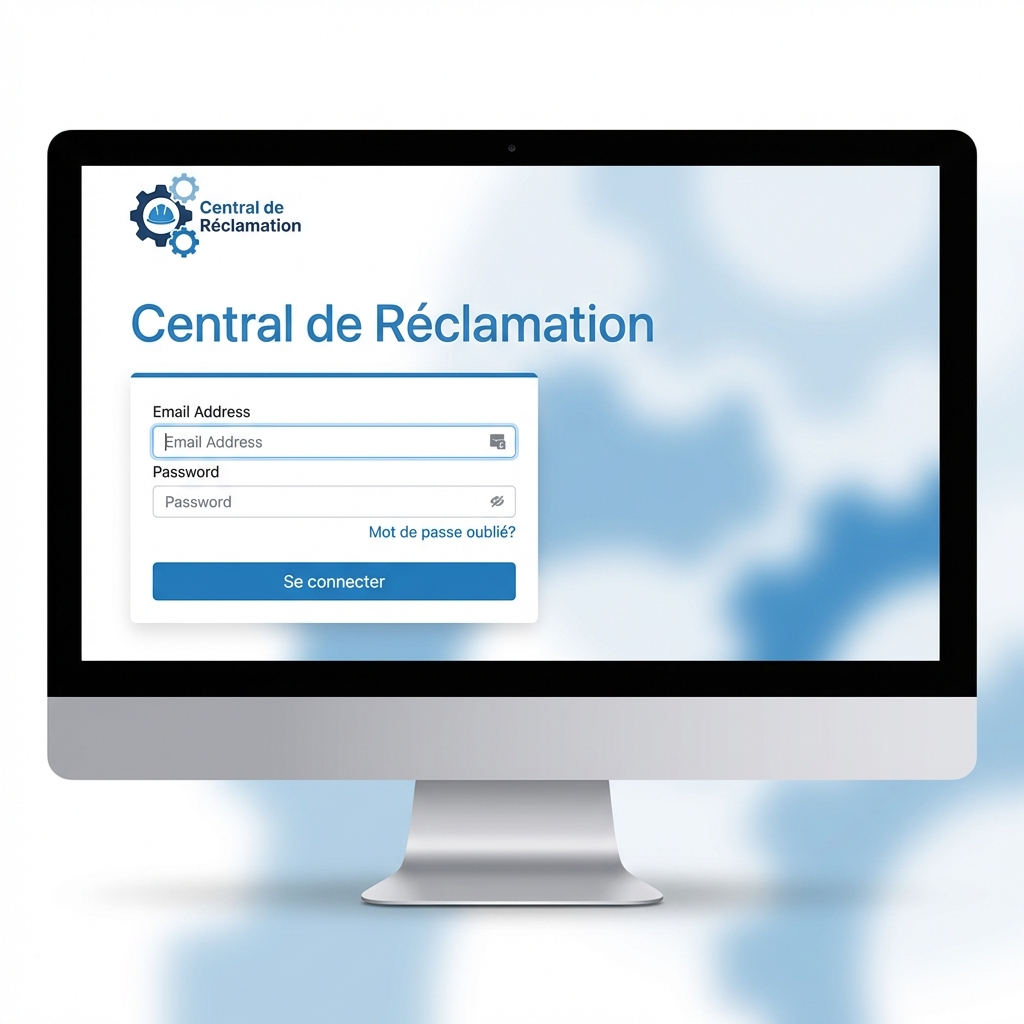
\includegraphics[width=14cm]{images/accueil_client.png}
    \caption{Interface d'accueil -- Page principale du système}
    \label{fig:accueil}
\end{figure}

\subsubsection{Formulaire de Nouvelle Réclamation}
Le formulaire de soumission permet au client de saisir les informations détaillées de sa réclamation, incluant la possibilité d'ajouter plusieurs produits et des pièces jointes.

\begin{figure}[H]
    \centering
    \fbox{\parbox{12cm}{\centering\vspace{3cm}\textit{Capture d'écran à insérer}\\[0.5cm]\texttt{images/form_nouvelle_reclamation.png}\vspace{3cm}}}
    \caption{Formulaire de création d'une nouvelle réclamation}
    \label{fig:form-reclamation}
\end{figure}

\subsubsection{Tableau de Bord Client}
Le dashboard client offre une vue centralisée de toutes les réclamations soumises avec leur statut actuel.

\begin{figure}[H]
    \centering
    \fbox{\parbox{12cm}{\centering\vspace{3cm}\textit{Capture d'écran à insérer}\\[0.5cm]\texttt{images/dashboard_client.png}\vspace{3cm}}}
    \caption{Tableau de bord de l'espace client}
    \label{fig:dashboard-client}
\end{figure}

% ==================================================
% ESPACE COMMERCIAL
% ==================================================
\subsection{Espace Commercial}

\subsubsection{Tableau de Bord Commercial}
L'interface commerciale permet aux agents de créer des réclamations au nom des clients et de suivre l'ensemble des tickets.

\begin{figure}[H]
    \centering
    \fbox{\parbox{12cm}{\centering\vspace{3cm}\textit{Capture d'écran à insérer}\\[0.5cm]\texttt{images/dashboard_commercial.png}\vspace{3cm}}}
    \caption{Tableau de bord de l'espace commercial}
    \label{fig:dashboard-commercial}
\end{figure}

% ==================================================
% ESPACE RMQ
% ==================================================
\subsection{Espace Responsable Management Qualité (RMQ)}

\subsubsection{Tableau de Bord RMQ}
Le tableau de bord RMQ permet une supervision globale des réclamations. Il affiche :
\begin{itemize}
    \item Des indicateurs statistiques en temps réel (KPI).
    \item La répartition des tickets par statut.
    \item La liste des derniers tickets reçus avec actions rapides.
\end{itemize}

\begin{figure}[H]
    \centering
    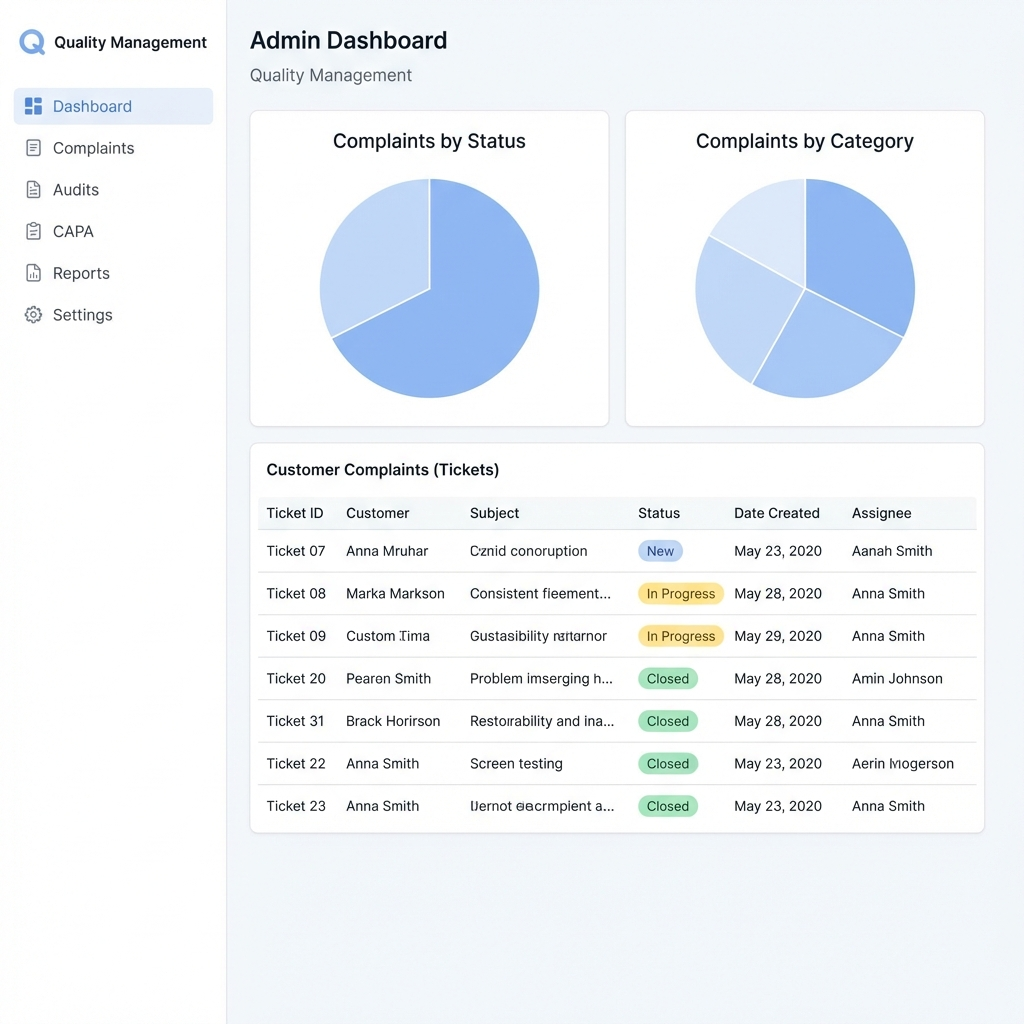
\includegraphics[width=14cm]{images/dashboard_rmq.png}
    \caption{Tableau de bord de gestion des réclamations -- Espace RMQ}
    \label{fig:dashboard-rmq}
\end{figure}

\subsubsection{Détail d'un Ticket}
Cette interface présente l'ensemble des informations d'une réclamation avec les actions disponibles (validation, refus, assignation fournisseur, changement de statut).

\begin{figure}[H]
    \centering
    \fbox{\parbox{12cm}{\centering\vspace{3cm}\textit{Capture d'écran à insérer}\\[0.5cm]\texttt{images/detail_ticket_rmq.png}\vspace{3cm}}}
    \caption{Interface de détail d'un ticket -- Espace RMQ}
    \label{fig:detail-rmq}
\end{figure}

\subsubsection{Module Statistiques}
Le module statistiques offre des graphiques et tableaux de bord analytiques pour le suivi des performances.

\begin{figure}[H]
    \centering
    \fbox{\parbox{12cm}{\centering\vspace{3cm}\textit{Capture d'écran à insérer}\\[0.5cm]\texttt{images/statistiques_rmq.png}\vspace{3cm}}}
    \caption{Module statistiques -- Espace RMQ}
    \label{fig:stats-rmq}
\end{figure}

% ==================================================
% ESPACE AQF
% ==================================================
\subsection{Espace Assistant Qualité Fournisseur (AQF)}

\subsubsection{Tableau de Bord AQF}
L'interface AQF affiche uniquement les tickets ayant un fournisseur assigné, permettant un suivi ciblé des réclamations liées aux fournisseurs.

\begin{figure}[H]
    \centering
    \fbox{\parbox{12cm}{\centering\vspace{3cm}\textit{Capture d'écran à insérer}\\[0.5cm]\texttt{images/dashboard_aqf.png}\vspace{3cm}}}
    \caption{Tableau de bord de l'espace AQF}
    \label{fig:dashboard-aqf}
\end{figure}

% ==================================================
% ESPACE ADMIN
% ==================================================
\subsection{Espace Administrateur}

\subsubsection{Gestion des Utilisateurs}
L'interface d'administration permet la gestion complète des utilisateurs du système (création, modification, activation/désactivation).

\begin{figure}[H]
    \centering
    \fbox{\parbox{12cm}{\centering\vspace{3cm}\textit{Capture d'écran à insérer}\\[0.5cm]\texttt{images/gestion_users_admin.png}\vspace{3cm}}}
    \caption{Interface de gestion des utilisateurs -- Espace Admin}
    \label{fig:admin-users}
\end{figure}

% ==================================================
% TESTS
% ==================================================
\section{Scénarios de Test}
Nous avons validé le fonctionnement via les tests fonctionnels suivants :

\begin{table}[H]
\centering
\begin{tabular}{|l|l|l|}
\hline
\textbf{Module} & \textbf{Action} & \textbf{Résultat Attendu} \\ \hline
Authentification & Saisir identifiants valides & Redirection vers Dashboard \\ \hline
Authentification & Saisir mot de passe incorrect & Message d'erreur affiché \\ \hline
Création Ticket & Envoyer formulaire vide & Blocage (Validation JS) \\ \hline
Création Ticket & Soumettre réclamation valide & Ticket créé + Email envoyé \\ \hline
Upload & Fichier invalide (.exe) & Rejet du fichier \\ \hline
Upload & Image valide (.jpg, .png) & Fichier enregistré \\ \hline
Validation RMQ & Valider un ticket & Statut mis à jour + Notification \\ \hline
Assignation & Assigner un fournisseur & Ticket visible dans AQF \\ \hline
\end{tabular}
\caption{Synthèse des tests fonctionnels réalisés}
\label{tab:tests}
\end{table}

\section{Sécurité}
Plusieurs mesures de sécurité ont été implémentées :
\begin{itemize}
    \item \textbf{Authentification :} Mots de passe hashés avec \texttt{password\_hash()}.
    \item \textbf{Sessions :} Gestion sécurisée des sessions PHP.
    \item \textbf{Requêtes préparées :} Utilisation de PDO pour prévenir les injections SQL.
    \item \textbf{Validation :} Contrôle des entrées utilisateur côté client et serveur.
    \item \textbf{Upload :} Restriction des types de fichiers autorisés.
\end{itemize}

\section*{Conclusion}
La phase de réalisation a permis de transformer les spécifications fonctionnelles et techniques en une application concrète et utilisable. L'architecture MVC et le choix des technologies ont facilité le développement d'une solution modulaire et évolutive. Les tests effectués confirment que le système est robuste et répond aux attentes initiales de la société SCPC Comptoir Hammami.
